\section{CID Design}
\label{sec:method}

CID is designed around two practical goals: improve task quality by allowing external evidence to correct uncertain or stale model state as soon as it becomes available, and improve end-to-end efficiency by overlapping external work with useful denoising while avoiding duplicate tool execution and unnecessary recomputation. The architecture follows from three corresponding requirements. First, exact externally supplied information must remain stable even while model cognition is revised. Second, an information need should become actionable before the model has fully serialized a textual or JSON tool call, so external latency can start earlier. Third, once a result has arrived, the model should be able to keep using or reinterpret it without repeatedly executing the same external operation. The components below implement these requirements jointly and integrate tool use directly into the ongoing generation process. Table~\ref{tab:cid-mechanisms} maps the six design requirements in Section~2.6 to the corresponding CID mechanisms and summarizes their intended effects.

Given a task prompt $P$, at diffusion update $s$, \cid maintains
\begin{equation}
  \mathcal{S}_s = (F_s, T_s, Y_s, \mathcal{B}_s, \mathcal{J}_s),
  \label{eq:cid-state}
\end{equation}
where $F_s$ is the fact channel, $T_s$ the thought channel, $Y_s$ the display channel, $\mathcal{B}_s$ the active perceptual bindings, and $\mathcal{J}_s$ the in-flight external jobs. The original prompt $P$ remains fixed token-level conditioning across the trajectory and sits outside the three mutable channels; explicitly protected prompt content may additionally be represented in $F_s$. The model updates $T_s$ and $Y_s$, while the environment and runtime update $F_s$, $\mathcal{B}_s$, and $\mathcal{J}_s$ under explicit permissions.

This separation makes ownership explicit. Externally controlled values need not be regenerated and therefore cannot silently drift during denoising, while cognition and display remain revisable. Keeping bindings and in-flight jobs in the same system state also lets external work advance without stopping the model trajectory.

\paragraph{Running Example.}

Consider a user who asks the model to compare two recently released systems and cite exact latency numbers from their documentation. At the start of generation, the model can already organize parts of the answer that do not depend on retrieval: it may identify the comparison dimensions, reserve display regions for evidence, and keep the numerical claims unresolved. During the same denoising process, a region of $T_s$ can begin to represent a need for the latency specification of the first system. This need can become useful to the runtime before the model has produced a complete textual request such as a search query or JSON call.

Once the intent adapter assigns sufficient probability to a registered documentation source and enough arguments are bound, the runtime creates a perceptual binding and launches the read asynchronously. Model denoising continues while the read is in flight. The thought state can refine the comparison plan, and the display state can develop stable material whose correctness does not depend on the missing number. Cells that depend on unavailable evidence remain uncertain until evidence arrives, avoiding guesses caused solely by generation progress.

Suppose the documentation then returns an exact latency of 37~ms. The runtime stores the returned value together with its provenance and version information. Policy may promote the exact value to the fact channel when it must be preserved verbatim. The percept encoder simultaneously constructs a projection conditioned on the current thought and display states. A numerical claim cell can become grounded in 37~ms, a tentative hypothesis that assumed a lower latency can reopen, and an already drafted comparison sentence can be revised during subsequent display denoising. These changes can occur within the same evolving trajectory because the observation directly conditions its current state.

If the answer continues to rely on the same specification, the binding stays active. Later denoising updates can re-project the cached 37~ms value without reading the documentation again, preserving its cognitive influence while the surrounding argument changes. If the source is versioned and a newer document appears, the same binding can request an external refresh and assimilate the new value. When the information need becomes inactive and its dependent output is stable, the runtime retires the binding. This example separates four events that conventional tool interfaces often collapse into one textual call: the emergence of a need, binding to a source, arrival of an external value, and continued cognitive use of that value.

\subsection{Three Coupled Channels}
\label{sec:channels}

\paragraph{Fact Channel.}
$F_s$ contains information whose value is controlled outside the generative state. The model can attend to it but cannot overwrite it. Importantly, this does not imply temporal immutability:
\begin{equation}
  F_{s+1} = \operatorname{ExternalUpdate}(F_s, e_{s+1}).
  \label{eq:fact-update}
\end{equation}
A clock, system load, changing document, or user-updated constraint may therefore change between diffusion steps. The channel may contain user-pinned statements, exact values that must be quoted, authoritative tool results, and provenance metadata. Not every tool result must be promoted to $F_s$; ephemeral or low-value observations may remain in the runtime cache and enter cognition only through a temporary projection. In the implementation, this permission is declared by the registered source descriptor rather than predicted by the generative model: a source may mark its returned observations as protected, and only the runtime performs the corresponding fact-store update.

This channel provides grounding while leaving reasoning to the mutable cognitive state. Separating protected values from mutable cognition prevents exact numbers, constraints, and provenance from being altered by later denoising, while external updates can still replace them when the underlying source genuinely changes. This directly targets factual and copying errors without freezing the rest of the model state.

Each fact item is represented as
\begin{equation}
  f_j = (v_j, \kappa_j, t_j, \nu_j, p_j),
\end{equation}
where $v_j$ is the value, $\kappa_j$ its source type, $t_j$ a timestamp, $\nu_j$ a version or freshness marker, and $p_j$ provenance. Fact-channel policy is an explicit runtime decision governing whether a tool result is promoted. The model can request or consume a source, but it has no output head that can directly write or promote a value into $F_s$.

\paragraph{Thought Channel.}
The thought channel is a structured cognitive field $T_s=(c_{s,1},\ldots,c_{s,N})$, with semantic matrix $H_s\in\mathbb{R}^{N\times d}$ whose row $i$ is $h_{s,i}$. It contains reasoning, hypotheses, information needs, tool intentions, percept interpretations, plans, constraints, and conclusions. Unlike text scratchpads or untyped hidden caches, it exposes structured mutable state through a stable model--runtime contract.

Making these states explicit gives the runtime something more useful than a partially generated string to act on. In particular, it can detect an information need, track which regions depend on it, and preserve uncertainty while a result is still in flight. This enables earlier tool execution and more selective revision after the result arrives.

\paragraph{Display Channel.}
$Y_s$ is a length-$L$ sequence over $\mathcal{V}\cup\{\textsc{mask}\}$ that converges to the user-visible output. It may be revised as $T_s$ changes. Display properties such as realized output length (e.g., the current EOS position or populated span), remaining budget, formatting constraints, and citation coverage can be fed back into the thought channel, allowing the model to adjust content continuously throughout generation.

Separating display from thought lets CID revise user-visible text when new evidence arrives without requiring all intermediate cognition to be serialized into that text. It also allows already useful parts of the answer to continue converging while evidence-dependent regions remain uncertain, preserving useful computation during tool latency.

The model performs coupled updates
\begin{align}
  T_{s+1} &\sim D_T(T_s \mid P, F_s, Y_s, \mathcal{P}_s, \tau^T_s), \\
  Y_{s+1} &\sim D_Y(Y_s \mid P, F_s, T_{s+1}, \tau^Y_s),
  \label{eq:coupled-denoise}
\end{align}
where $\mathcal{P}_s$ denotes perceptual projections from active bindings and $\tau^T_s,\tau^Y_s$ are local editability schedules for thought cells and display positions, respectively. For $Y_s$, increased editability can be realized by remasking or bounded revision of already visible tokens.

\subsection{Typed Cognitive Tensor}
\label{sec:tct}

The thought channel is organized as a \emph{Typed Cognitive Tensor} (\tct), whose dense semantic core is $H_s$, with aligned per-cell typed fields carrying symbolic and runtime information. Cognitive cell $i$ is
\begin{equation}
  c_{s,i} = (h_{s,i}, r_{s,i}, a_{s,i}, q_{s,i}, u_{s,i}, \tau_{s,i}, \ell_{s,i}),
  \label{eq:cognitive-cell}
\end{equation}
with the following fields:
\begin{itemize}[leftmargin=*]
  \item $h_{s,i}\in\mathbb{R}^d$: continuous semantic content;
  \item $r_{s,i}$: a soft role distribution, such as hypothesis, information need, percept, plan, constraint, or conclusion;
  \item $a_{s,i}$: sparse symbolic anchors, including tool identifiers, entities, paths, numeric values, schema fields, or output spans;
  \item $q_{s,i}$: links to fact items, bindings, or other cognitive cells;
  \item $u_{s,i}$: epistemic or binding uncertainty;
  \item $\tau_{s,i}$: a local diffusion level controlling editability;
  \item $\ell_{s,i}$: lifecycle state, such as active, waiting, stable, or retired.
\end{itemize}

\begin{figure}[htbp]
  \centering
  \resizebox{0.98\columnwidth}{!}{\begin{tikzpicture}[cid figure,
  field/.style={draw=figline, line width=0.6pt, rounded corners=3pt,
    font=\sffamily\footnotesize, minimum height=0.72cm, text width=2.88cm, inner sep=4pt, align=center},
  label/.style={font=\sffamily\scriptsize, anchor=west}]
  % Aligned fields communicate a structured cell without implying dataflow.
  \node[anchor=west,font=\sffamily\small\bfseries] at (0,0.4) {Cognitive cell $c_{s,i}$};
  \node[field,cid thought,text width=6.30cm,minimum height=0.9cm,anchor=west] at (0,-0.38)
    {$h_{s,i}\in\mathbb{R}^d$\quad Semantic content};
  \node[field,cid thought,anchor=west] at (0,-1.35) {$r_{s,i}$\\Soft role};
  \node[field,cid fact,anchor=west] at (3.42,-1.35) {$a_{s,i}$\\Symbolic anchors};
  \node[field,cid fact,anchor=west] at (0,-2.35) {$q_{s,i}$\\Source / cell links};
  \node[field,cid runtime,anchor=west] at (3.42,-2.35) {$u_{s,i}$\\Uncertainty};
  \node[field,cid runtime,anchor=west] at (0,-3.35) {$\tau_{s,i}$\\Local diffusion};
  \node[field,cid display,anchor=west] at (3.42,-3.35) {$\ell_{s,i}$\\Lifecycle};
\end{tikzpicture}
}
  \caption{Structure of a Typed Cognitive Tensor cell.}
  \label{fig:tct-anatomy}
\end{figure}

Roles are soft and may overlap. A cell can simultaneously represent a hypothesis and the information need that would verify it. Sparse anchors prevent precise objects from drifting in a continuous latent space, while the continuous component preserves ambiguity and multiple competing interpretations.

These fields are included because different parts of tool-augmented reasoning require different behavior. Soft roles retain the flexibility of continuous cognition; symbolic anchors preserve exact tool identifiers, entities, paths, numbers, and output locations; source links identify which state should be revised when evidence changes; uncertainty exposes whether an external result is still needed; and per-cell diffusion levels allow revision to concentrate on affected regions. The expected benefit is higher grounding accuracy with less destructive or global recomputation after each external event.

The local noise vector
\begin{equation}
  \boldsymbol{\tau}_s = (\tau_{s,1},\ldots,\tau_{s,N})
\end{equation}
allows different regions to evolve asynchronously. A supported conclusion may be nearly stable, an unresolved query may remain highly diffused, and a previously stable hypothesis may be reopened after a changing external fact arrives.

\subsection{Latent Information Needs}
\label{sec:latent-needs}

Tool use is represented as a role within $T_s$, not as a separate text region. A model-side intent adapter reads the cognitive field and registered source descriptors $\mathcal{D}=\{d_m\}$:
\begin{equation}
  I_s = G_{\phi}(T_s, Y_s, \mathcal{D}).
  \label{eq:intent-adapter}
\end{equation}
Each candidate need $i_k\in I_s$ contains
\begin{equation}
  i_k = (n_k, \pi_k, \alpha_k, \omega_k, \eta_k, \chi_k),
\end{equation}
where $n_k$ is a continuous need embedding, $\pi_k$ a distribution over registered sources or tools, $\alpha_k$ partially bound arguments, $\omega_k$ uncertainty, $\eta_k$ freshness or persistence demand, and $\chi_k$ links to affected cognitive or display regions. The implementation assigns each owning cognitive cell a small number of stable need slots. A slot's latent query is used jointly for source selection and for learned routing over live TCT cells and display positions. Thresholded cell scores and contiguous display-position scores materialize $\chi_k$; the owning cell is always retained, while one need may additionally target several other cells and display spans without being duplicated into separate bindings.

The adapter exposes a typed interface over the cognitive field. This choice preserves early access to latent intent while insulating the runtime from model-specific hidden-state geometry. It also separates three stages that need not occur at the same diffusion step:
\begin{equation}
  \begin{aligned}
    \text{need emergence} &\rightarrow \text{source selection}\\
                          &\rightarrow \text{argument binding}.
  \end{aligned}
\end{equation}
For read-only tools, a binding may begin before every argument has reached textual certainty, provided the source accepts approximate or progressively refined selectors.

\begin{figure*}[t]
  \centering
  \resizebox{0.96\textwidth}{!}{\begin{tikzpicture}[
  cid figure,
  state/.style={draw=figline, line width=0.65pt, rounded corners=3pt, minimum height=0.82cm, align=center, inner xsep=8pt, inner ysep=4pt},
  flow/.style={-{Latex[length=1.8mm]}, thick},
  loop/.style={-{Latex[length=1.8mm]}, thick, dashed},
  note/.style={font=\sffamily\footnotesize, align=center}
]
  % Position each state from the previous node's actual border so all four
  % horizontal arrows have the same visible length even when text widens a box.
  \node[state, cid thought, minimum width=2.25cm] (need) at (0,0) {active\\information need};
  \node[state, cid runtime, minimum width=2.35cm, right=0.75cm of need] (bind) {persistent binding\\$b_j$};
  \node[state, cid fact, minimum width=2.5cm, right=0.75cm of bind] (cache) {cached value\\version + provenance};
  \node[state, cid thought, minimum width=2.45cm, right=0.75cm of cache] (project) {contextual projection\\$P_j^s$};
  \node[state, cid display, minimum width=2.35cm, right=0.75cm of project] (state) {evolving\\thought + display};

  \draw[flow] (need) -- (bind);
  \draw[flow] (bind) -- (cache);
  \draw[flow] (cache) -- (project);
  \draw[flow] (project) -- (state);

  \node[state, minimum width=2.05cm, below=1.18cm of bind] (retire) {retire binding};
  \draw[flow] (bind.south) -- node[note, right] {need inactive} (retire.north);

  \node[state, cid fact, minimum width=2.6cm, below=1.18cm of cache] (source) {external read\\or refresh};
  \draw[flow] (source.north) -- (cache.south);
  \node[note] at ($(source.south)+(0,-0.42)$) {first fetch or source-version change};

  \draw[loop] (state.north) -- ++(0,1.0) -| (project.north);
  \node[note] at ($(project.north)!0.5!(state.north)+(0,1.38)$) {need remains active:\\re-project cached value};
\end{tikzpicture}
}
  \caption{Lifecycle of a persistent perceptual binding.}
  \label{fig:binding-lifecycle}
\end{figure*}

The main efficiency benefit is that external work can start at need emergence or partial argument binding, before a complete call has been decoded. If the need is identified several denoising steps earlier than an executable textual call, those steps can overlap tool latency and reduce its contribution to the critical path. At the same time, retaining uncertainty and partial arguments avoids forcing the model to commit prematurely to details that later denoising may change.

\subsection{Persistent Perceptual Bindings}
\label{sec:bindings}

A conventional tool call is a transient request--response pair. CID instead creates a persistent perceptual binding
\begin{equation}
  b_j = (i_j, m_j, \alpha_j, \rho_j, z_j, \chi_j),
  \label{eq:binding}
\end{equation}
where $i_j$ is the originating need, $m_j$ the source or tool, $\alpha_j$ current arguments, $\rho_j$ a refresh policy, $z_j$ runtime cache and version state, and $\chi_j$ the affected thought and display regions.

A binding remains active while the corresponding information need remains active. Repeated intent is therefore not automatically treated as a redundant model failure. It can mean that the model wants the percept to remain cognitively salient. The runtime distinguishes two operations:
\begin{align}
  \text{external refresh: }& v_j^{s+1} \leftarrow m_j(\alpha_j, s+1), \\
  \text{cognitive refresh: }& P_j^{s+1} \leftarrow \Project(v_j, T_s, Y_s).
  \label{eq:two-refreshes}
\end{align}

\paragraph{Static or Unchanged Source.}
If the source version is unchanged, the runtime can reuse $v_j$ but recompute $P_j^{s+1}$. The same fact may therefore receive a different task-specific interpretation as cognition evolves. This supports copying and sustained reference: the source need not be re-read, yet its influence is renewed at each relevant denoising update.

\paragraph{Changing Source.}
If the source is time-varying or streamable, $\rho_j$ may request polling, version checks, event subscriptions, or incremental chunks. An arriving value updates a fact item when the runtime-owned source policy marks its results as protected, and always permits a new cognitive projection. Examples include current time, evolving realized display length, a modified file, sensor input, or streaming retrieval results.

A simple refresh policy is
\begin{equation}
  \rho_j(s)=
  \begin{cases}
    \textsc{reproject}, & \nu_j(s)=\nu_j(s-1),\\
    \textsc{refetch+reproject}, & \nu_j(s)\neq\nu_j(s-1),\\
    \textsc{sleep}, & \Pr(i_j\text{ active})<\delta.
  \end{cases}
  \label{eq:refresh-policy}
\end{equation}
Here $\nu_j(s)$ denotes a version already observed through a source event or a lightweight freshness probe; obtaining it is itself external work. If no cheap version signal exists, a due refresh must re-read the source because its version cannot be assumed to be known. More advanced policies can trade information gain, latency, and tool cost.

This distinction is what allows persistent information use without persistent I/O. For a static source, CID can repeatedly refresh the result's influence on evolving cognition while paying the external access cost only once. For a changing source, the same binding provides an explicit place to decide when a new fetch is worth its latency or cost. Persistent bindings therefore reduce duplicate calls while still allowing long or changing reasoning trajectories to remain grounded in external information.

\subsection{Perceptual Assimilation}
\label{sec:assimilation}

The percept encoder converts each tool result into a context-dependent projection
\begin{equation}
  P_j^s = E_{\psi}(v_j, p_j, T_s, Y_s),
  \label{eq:percept-projection}
\end{equation}
whose interpretation depends on the current thought and display states. Projection cells carry source links to $v_j$ when provenance matters. The thought denoiser integrates them with gated cross-attention or residual updates:
\begin{equation}
  \widetilde{T}_s = T_s + \sum_{j\in\mathcal{B}_s} g_{j,s}\,A(T_s,P_j^s),
  \label{eq:percept-assimilation}
\end{equation}
where $g_{j,s}$ is predicted from need persistence, relevance, and source freshness. This residual form is one realization of the $\mathcal{P}_s$ conditioning in \cref{eq:coupled-denoise}; an implementation may perform the same fusion inside $D_T$.

\begin{figure*}[t]
  \centering
  \resizebox{0.96\textwidth}{!}{% Vector source: scripts/draw_figures.py; editable interchange: runtime-loop.svg
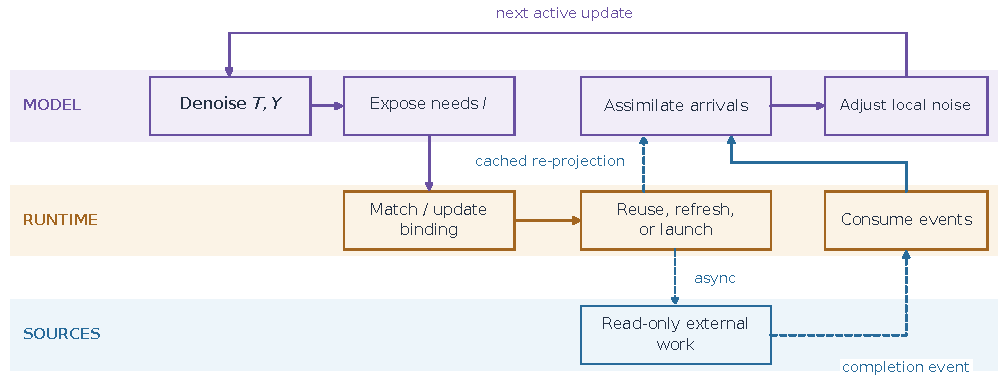
\includegraphics[width=0.96\textwidth]{figures/runtime-loop.pdf}
}
  \caption{CID runtime loop for read-only perception.}
  \label{fig:cid-runtime}
\end{figure*}

Recomputing the projection from the current $T_s$ and $Y_s$ lets one cached result support different parts of the reasoning as the trajectory evolves, without another external call. It also allows a newly arrived result to affect already formed hypotheses and display regions immediately, including content formed before the result arrived.

New evidence may change the editability of existing cells. Conceptually, let $\Delta_{j,i}$ estimate how strongly percept $j$ changes the posterior of cell $i$. A local update can be written as
\begin{equation}
  \tau_{s+1,i} = \operatorname{clip}
  \left(\tau_{s,i} + \lambda_{\mathrm{open}}\Delta^-_{j,i}
  - \lambda_{\mathrm{close}}\Delta^+_{j,i}\right),
  \label{eq:local-noise-update}
\end{equation}
where $\Delta^-_{j,i}$ denotes evidence favoring reopening and $\Delta^+_{j,i}$ evidence favoring stabilization. The current implementation does not instantiate separate support/conflict heads. Instead, the neural core directly predicts a bounded local-noise delta together with a \textsc{keep}, \textsc{reopen}, or \textsc{stabilize} action, and the runtime lifecycle gate applies the legal transition. Evidence-linked display positions are revised analogously through the learned $\chi_k$ routing, remasking, and bounded visible-token revision.

Local reopening is important for efficiency as well as correctness. New evidence should revise the state it invalidates, but it should not discard unrelated work that was already correct. Adjusting editability per cell therefore aims to preserve useful computation while concentrating additional denoising on regions that actually need correction.

\subsection{Asynchronous Runtime}
\label{sec:runtime}

\Cref{fig:cid-runtime} describes the runtime loop. Model denoising may continue while read-only work is outstanding, but only until a learned \emph{current-information equilibrium} signal fires. The runtime then pauses if required work remains and resumes on external progress; otherwise it forms a terminal candidate.

The runtime is asynchronous for a direct performance reason: waiting for retrieval, file I/O, or another read-only source should not automatically become idle model time. CID allows the model to refine source-independent cognition and display regions while the job is in flight, then revises dependent regions after arrival. End-to-end latency improves when this waiting-time computation remains useful, so the evaluation measures end-to-end latency at matched answer quality and treats token-generation speed as an insufficient metric on its own.

Initialization sets facts $F$, an initial thought state $T$, masked display $Y$, bindings $\mathcal{B}=\varnothing$, and jobs $\mathcal{J}=\varnothing$. Each model update exposes information needs; the runtime matches or updates bindings, launches a read when policy requires a fresh value and no equivalent job is active, consumes events, and re-projects cached values when external access is unnecessary. The model adjusts local noise until current-information equilibrium or a budget boundary; quiescent waiting consumes no model-update budget. Before termination, a freshness barrier completes required bindings and refreshes due values, with new evidence resuming refinement. External work is keyed by source and canonicalized arguments, and a completion applies only when an active binding still has the same work key, making obsolete work cancellable or discardable. Equivalent jobs are deduplicated without suppressing repeated perception: identical needs may share one cached value while receiving fresh projections. A refined need can update a binding's selector, while independent verification can establish another binding. The step cap bounds model updates; a separate wall-clock budget bounds the trajectory.

The same termination mechanism also provides a natural test-time compute control. When the learned equilibrium signal is thresholded, a deployment can raise its termination threshold to require stronger evidence of convergence, or lower it to permit earlier exit; the step and wall-clock caps provide complementary hard limits. This yields a runtime \emph{reasoning-effort} control without introducing a separate reasoning mode: easy instances may still terminate early, whereas unresolved states can consume more refinement steps up to the configured budget. Required bindings and the freshness barrier remain mandatory regardless of the selected effort level.

\medskip
\noindent\rule{\columnwidth}{0.5pt}
\vspace{3pt}
\noindent\textbf{TRAINING OBJECTIVE}\par\vspace{2pt}
CID requires a model trained for channel semantics and asynchronous events. A training trajectory contains a task $x$, protected facts $F$, tool/source descriptors $\mathcal{D}$, external event sequence $E=(e_1,\ldots,e_K)$ with arrival times, target thought structures $T^*$ or weak structural supervision, and final display $Y^*$.

Training randomizes event arrival, source freshness, and cache state. Before a needed event arrives, the model should maintain uncertainty, expose a binding need, and avoid fabricating the missing value. Waiting and final snapshots supervise the equilibrium signal; runtime state distinguishes quiescence from termination. After arrival, the model should assimilate the percept, revise affected cells, preserve unrelated cognition, and update the display.

A possible objective is
\begin{align}
  \mathcal{L} ={}& \mathcal{L}_{T}
  + \lambda_Y\mathcal{L}_{Y}
  + \lambda_I\mathcal{L}_{\mathrm{intent}}
  + \lambda_B\mathcal{L}_{\mathrm{bind}} \notag\\
  &+ \lambda_P\mathcal{L}_{\mathrm{assim}}
  + \lambda_{\chi}\mathcal{L}_{\mathrm{route}}
  + \lambda_R\mathcal{L}_{\mathrm{refresh}}
  + \lambda_G\mathcal{L}_{\mathrm{ground}}
  + \lambda_C\mathcal{L}_{\mathrm{conv}}.
  \label{eq:training-objective}
\end{align}
The first two terms train thought and display diffusion; the others train intent exposure, binding, affected-region routing, event-conditioned revision, refresh behavior, symbolic grounding, and the equilibrium signal. In the concrete neural contract, routing supervision is multi-label over live TCT cells and display positions for each stable need slot; contiguous positive display positions are materialized as spans at runtime. Fact promotion is intentionally excluded from the model loss because write permission to the protected fact channel is a runtime/source policy.

Static-copy training examples repeatedly expose an unchanged source while the output is gradually composed. Dynamic-monitoring examples change the source during denoising and require the thought and display states to track the latest externally supplied value. Search and file-reading examples teach need emergence, partial query binding, delayed arrival, and evidence-conditioned revision.
\par\vspace{3pt}
\noindent\rule{\columnwidth}{0.5pt}
\par
